\documentclass{templateNote}
\usepackage{tcolorbox}
\usepackage{tabularx}
\usepackage{hyperref}
\usepackage{amsmath}
\usepackage{amssymb}
\usepackage{pdflscape}
\usepackage{tikz}
\usepackage{pdfpages}
\usepackage{soul}
\usepackage{media9}
\usepackage{adjustbox}
\usepackage{pdfpages}
\usepackage[spanish,es-noquoting]{babel}

\begin{document}
\linklogoU{https://www.ubiobio.cl/w/}
\linklogoD{https://github.com/NicoGomezM}
\imagenlogoU{img/logo-ubb-txt-face.png}
\imagenlogoD{img/logoNGMFormal_sinF.png}
\titulo{Laboratorio 5:  Bloques digitales secuenciales}
\asignatura{Laboratorio Arquitectura de Computadores}
\autor{
    Nicolás \textsc{Gómez Morgado}
}

\portada
\margenes

\section{Actividades}
\subsection{Protoboard}
\begin{enumerate}
    \item Averigüe las características del circuito digital 74LS74. Destaque pines que identifican entradas de datos y salidas, VCC y GND. Señale bajo qué tipo de flanco el circuito toma en cuenta los valores de entrada.
    
    Para el circuito digital 74LS74, se tiene que es un circuito integrado que contiene dos flip-flops tipo D. Cada flip-flop tiene una entrada de datos (D), una entrada de reloj (CLK), una entrada de reset (R) y una entrada de set (S). Además, tiene una salida de Q y una salida de Q negada. El circuito toma en cuenta los valores de entrada en flanco de subida del reloj (CLK). Por lo tanto los pines de entrada para este tipo de circuito
        serian los pines 1,2,3,4,13,12,11,10 y los pines de salida serian los pines 5,6,9,8. Los pines VCC y GND son los pines 14 y 7 respectivamente.

        \begin{figure}[H]
            \centering
            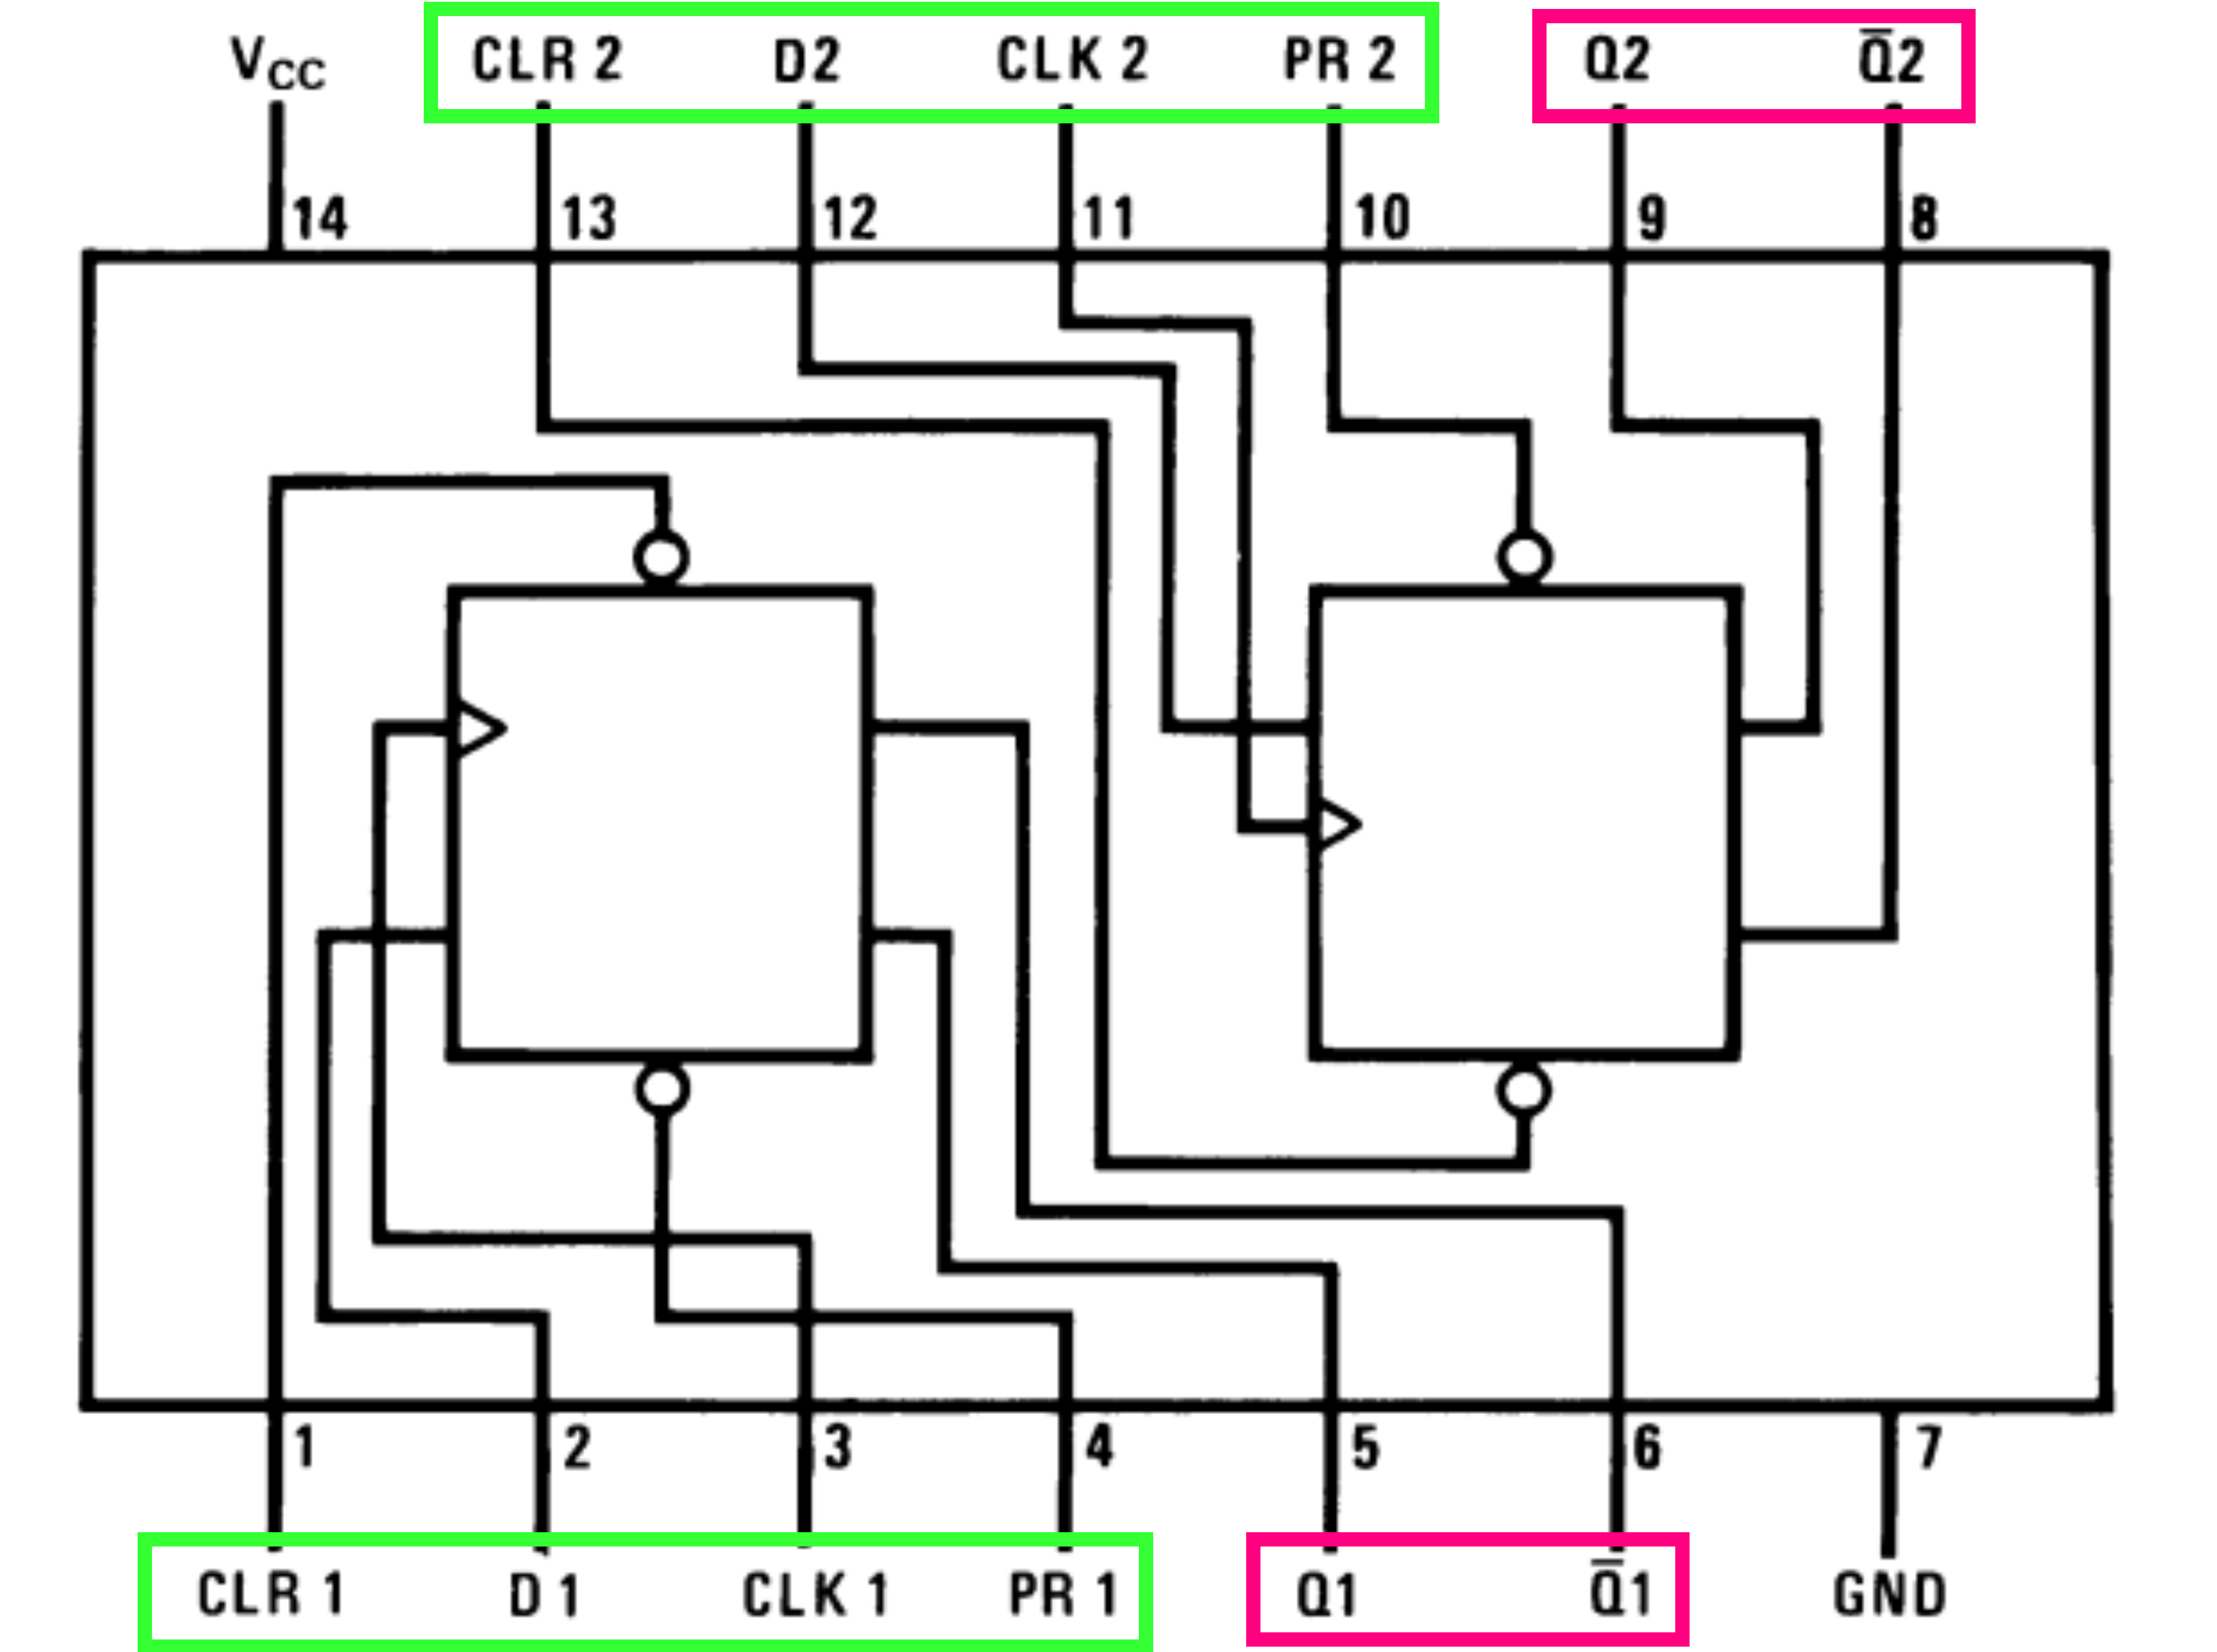
\includegraphics[width=0.5\textwidth]{img/entr-salid.png}
        \end{figure}
    
    \textbf{Para este circuito los pines remarcados con verde son de entrada y los pines remacados con rosa son de salida.}

    \item ¿Qué valores de los pines S y R son prohibidos y cuál es la razón de esto?
    
    Los valores prohibidos para los pines S y R son los valores 1 y 0 respectivamente. Esto se debe a que si se tiene un valor de 1 en el pin S, el flip-flop se pone en estado de set, lo que significa que la salida Q se pone en 1. Por otro lado, si se tiene un valor de 0 en el pin R, el flip-flop se pone en estado de reset, lo que significa que la salida Q se pone en 0. Por lo tanto, si se tiene un valor de 1 en S y un valor de 0 en R, se tendría una contradicción en el circuito, ya que la salida Q estaría en 1 y 0 al mismo tiempo.

    \item ¿Qué valores deben tener los pines S y R para que el circuito retenga el valor dado en la entrada D, tal que D sea igual a Q?
    
    Para que el circuito retenga el valor dado en la entrada D, tal que D sea igual a Q, los pines S y R deben tener un valor de 0. Esto se debe a que si se tiene un valor de 0 en el pin S, el flip-flop se pone en estado de set, lo que significa que la salida Q se pone en 1. Por otro lado, si se tiene un valor de 0 en el pin R, el flip-flop se pone en estado de reset, lo que significa que la salida Q se pone en 0. Por lo tanto, si se tiene un valor de 0 en S y un valor de 0 en R, se tendría que la salida Q se mantendría en el valor de la entrada D.
    
    \item Averigüe cual es la entrada del reloj (CLK). Utilice un switch del protoboard para simular esta señal.

    Para este circuito tenemos 2 entradas de reloj, una para cada flip-flop. La entrada de reloj para el primer flip-flop es el pin 3 y para el segundo flip-flop es el pin 11. Para simular esta señal se puede utilizar un switch del protoboard conectado a la entrada de reloj de cada flip-flop.
    
    \item Instale el circuito en protoboard y corrobore su funcionamiento validando su tabla de verdad. Explique en qué condiciones el circuito es capaz de “memorizar”. Corrobore que los cambios de estado ocurren en un flanco. Adjuntar circuito protoboard para revisión (constructor Virtual, Tinkercad o foto Protoboard real).
    
    \begin{figure}[H]
        \centering
        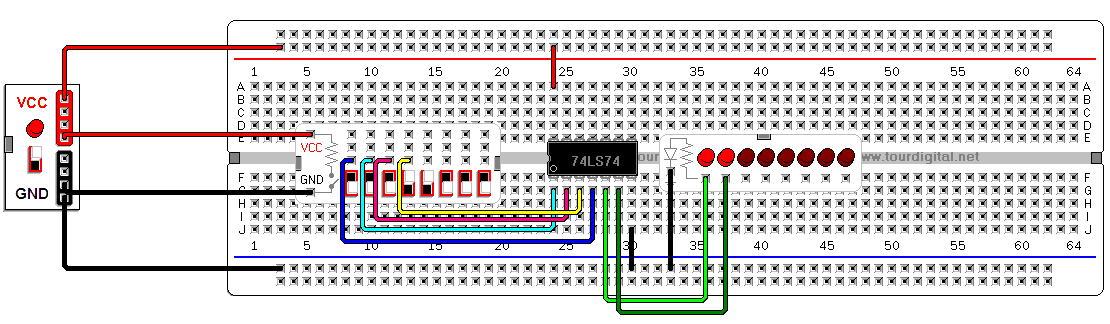
\includegraphics[width=0.8\textwidth]{img/circuito.png}        
    \end{figure}

    Para el circuito de la figura anterior, se tiene que el circuito es capaz de memorizar cuando los pines S y R tienen un valor de 0. Esto se debe a que si se tiene un valor de 0 en el pin S, el flip-flop se pone en estado de set, lo que significa que la salida Q se pone en 1. Por otro lado, si se tiene un valor de 0 en el pin R, el flip-flop se pone en estado de reset, lo que significa que la salida Q se pone en 0. Por lo tanto, si se tiene un valor de 0 en S y un valor de 0 en R, se tendría que la salida Q se mantendría en el valor de la entrada D.

\end{enumerate}

\newpage
\subsection{Logisim}
\begin{enumerate}
    \item Busque el circuito correspondiente a un registro (register). Verifique que este se configure para almacenar palabras de 4 bits, pegar capturas.
    
    \begin{figure}[H]
        \centering  
        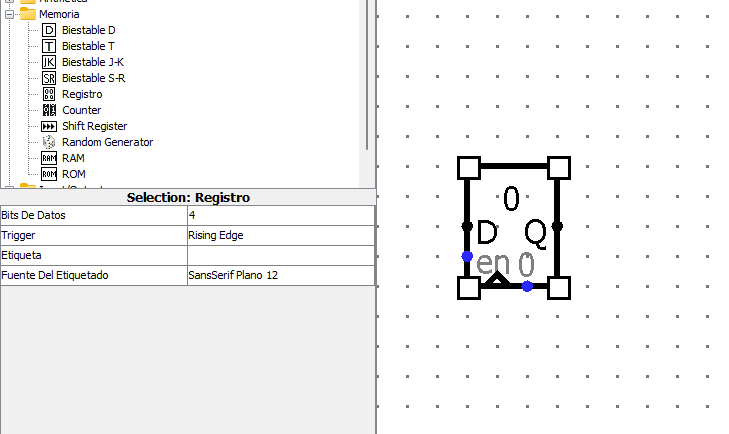
\includegraphics[width=0.8\textwidth]{img/regisstro.png}
    \end{figure}

    \item Realice el experimento que se muestra en video: \\https://www.youtube.com/watch?v=384-g7T5JwU. \\Pruebe con distintos valores de entrada y con distintos tipos de flanco y pegar capturas.
    
    \begin{figure}[H]
        \centering
        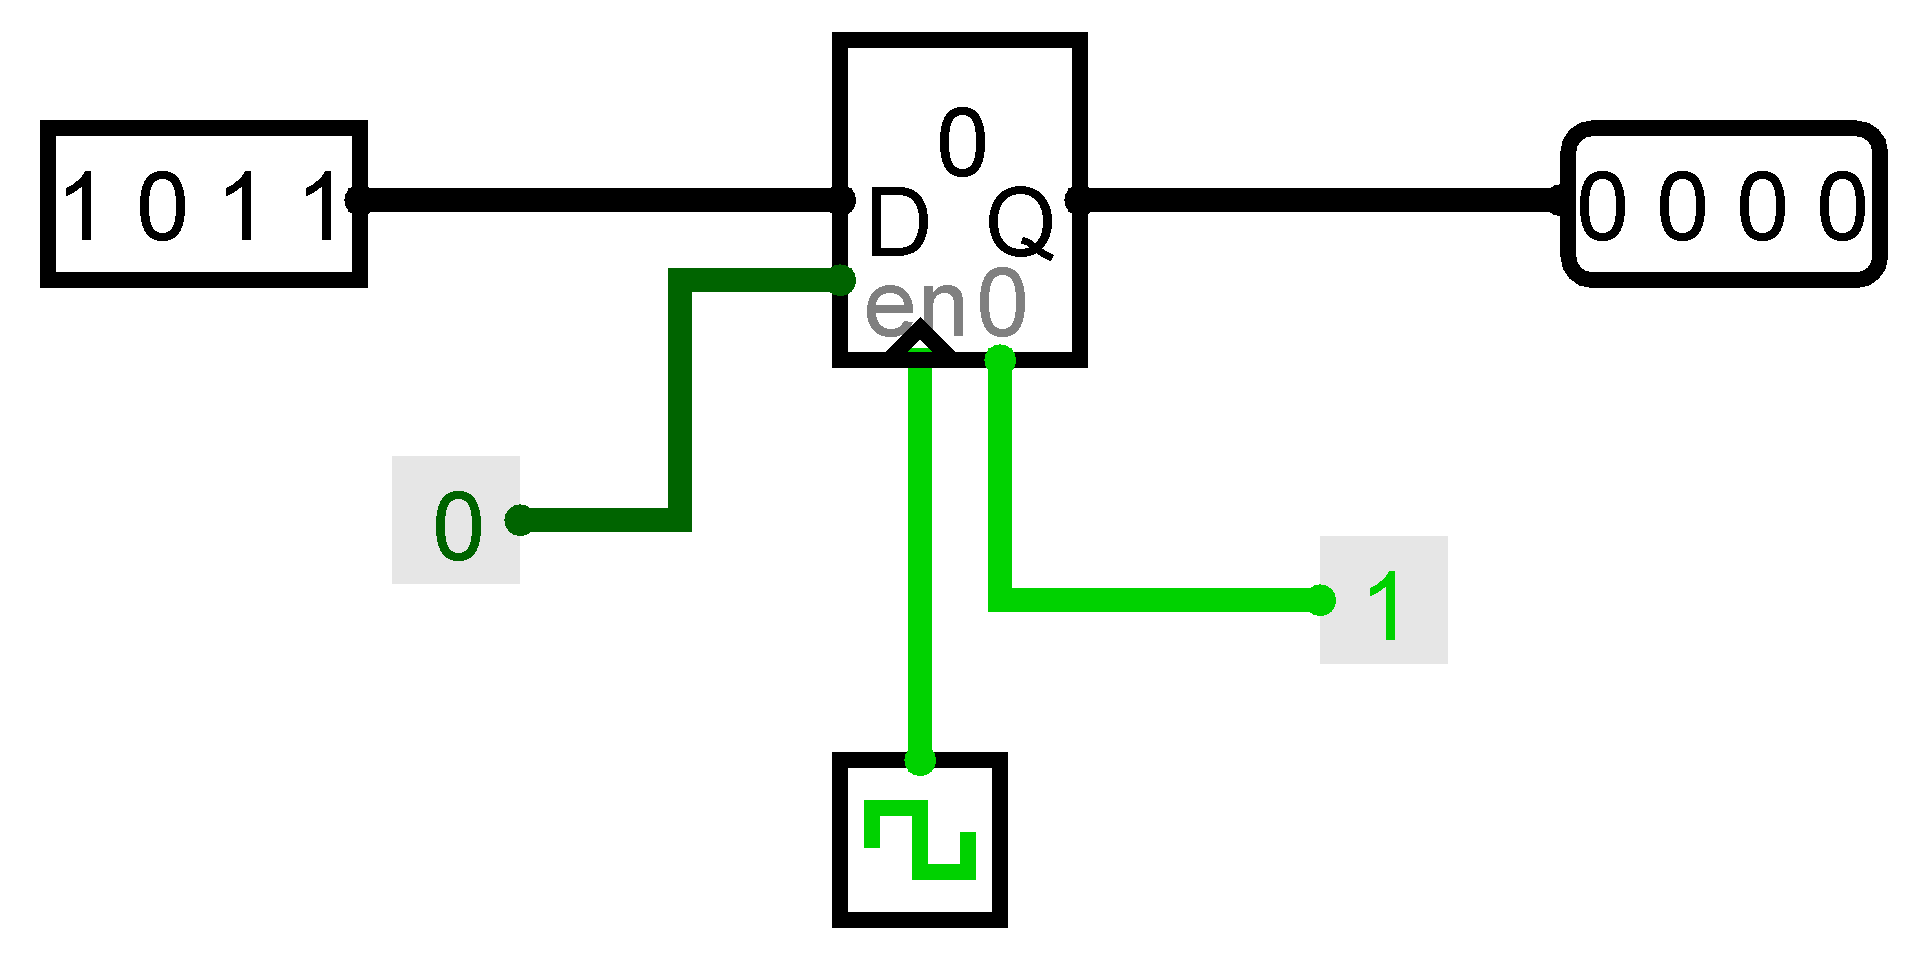
\includegraphics[width=0.6\textwidth]{img/primertry.png}
        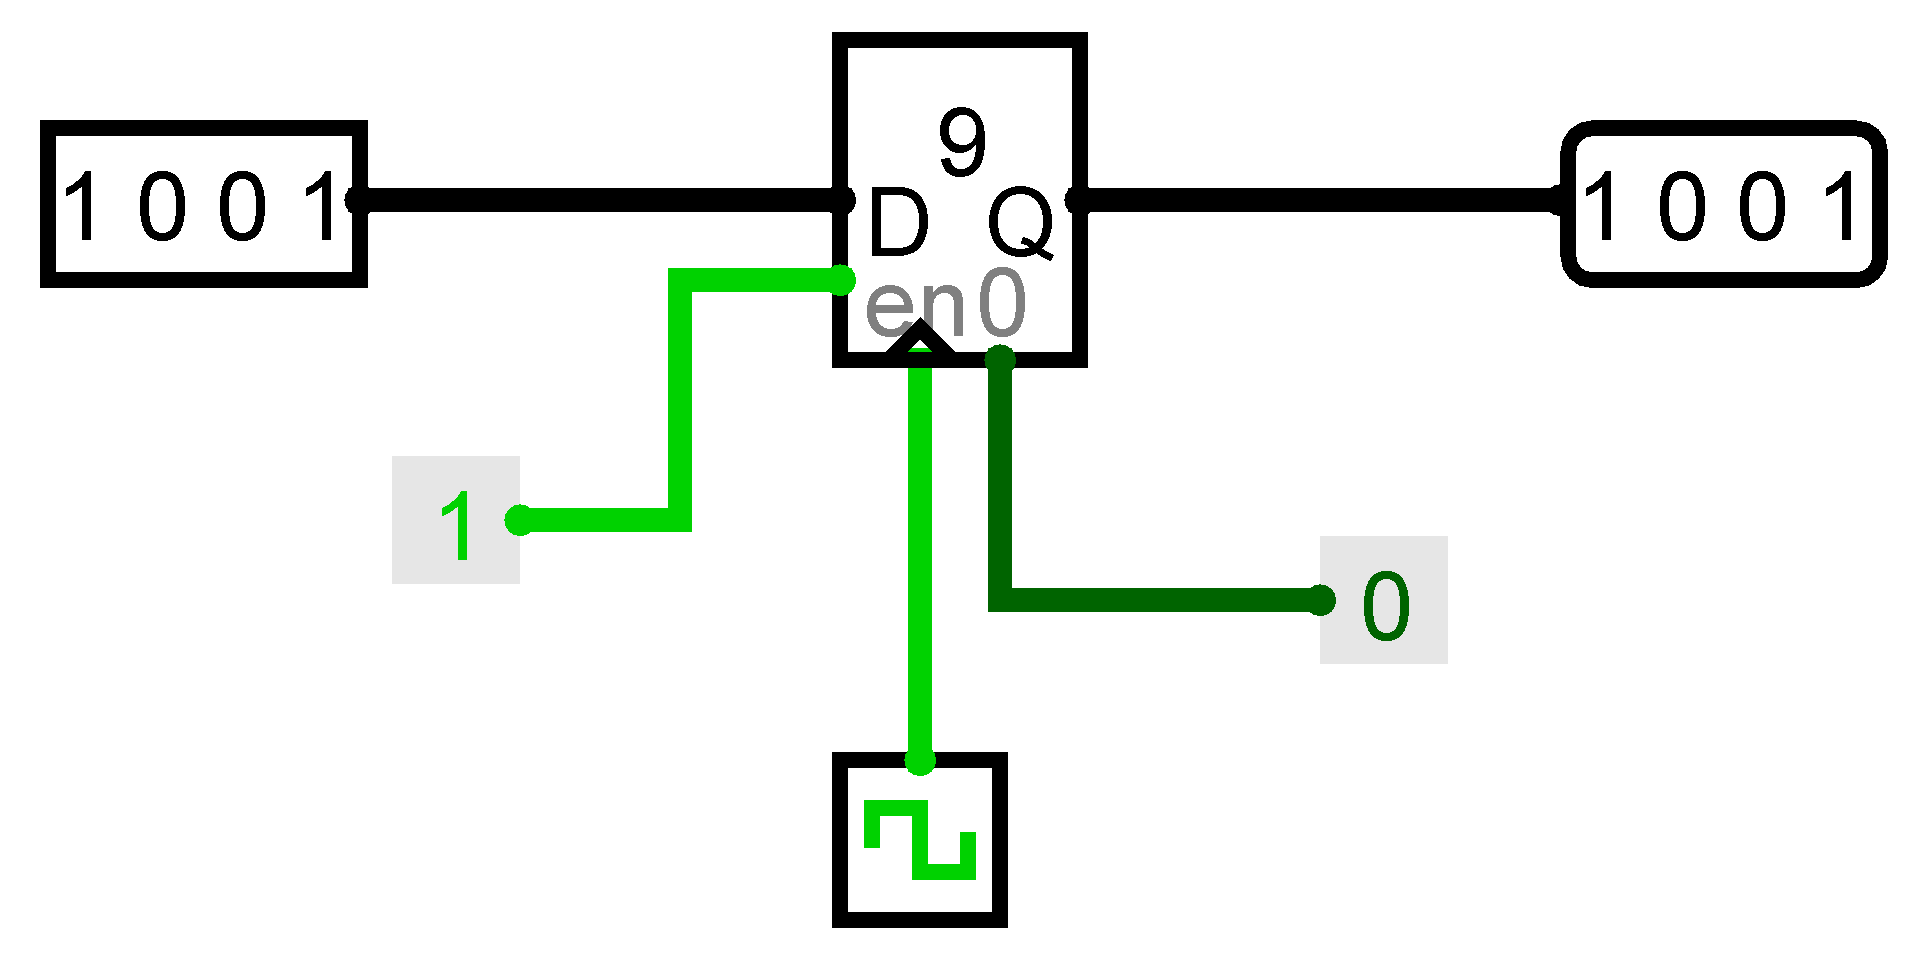
\includegraphics[width=0.6\textwidth]{img/segundotry.png}
    \end{figure}

    \newpage
    \begin{figure}[H]
        \centering
        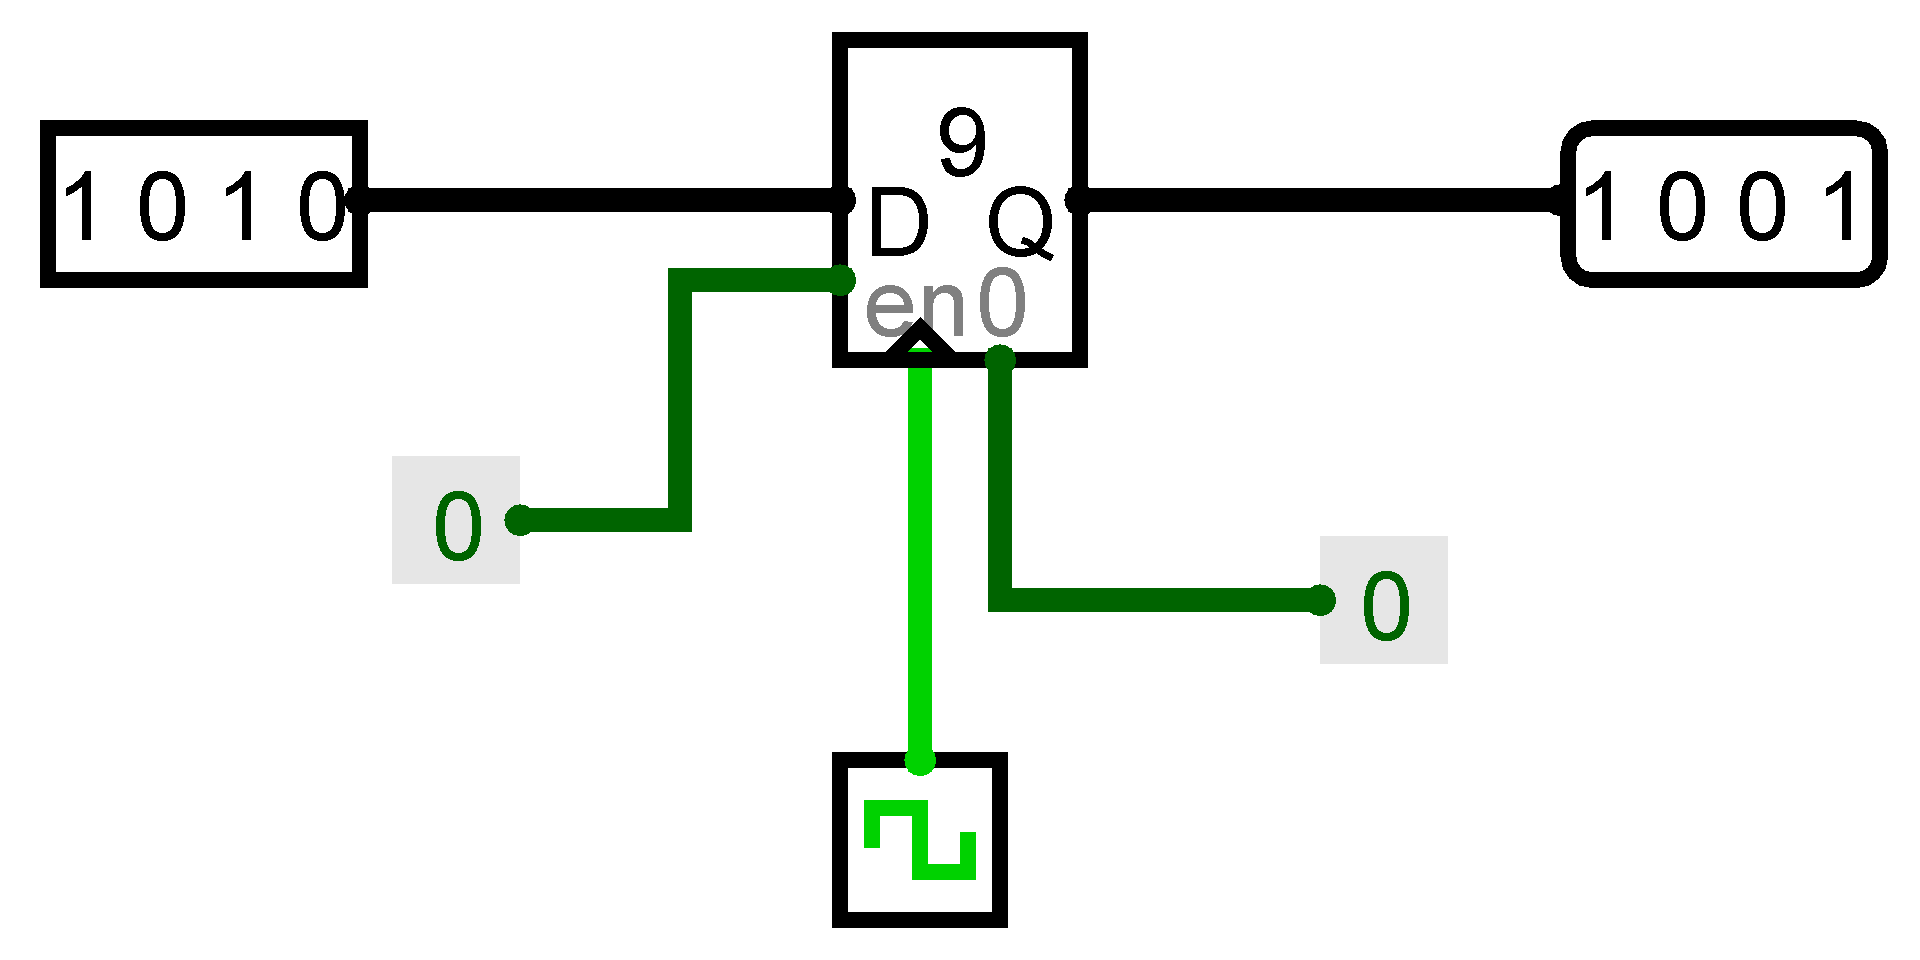
\includegraphics[width=0.6\textwidth]{img/tercertry.png}
        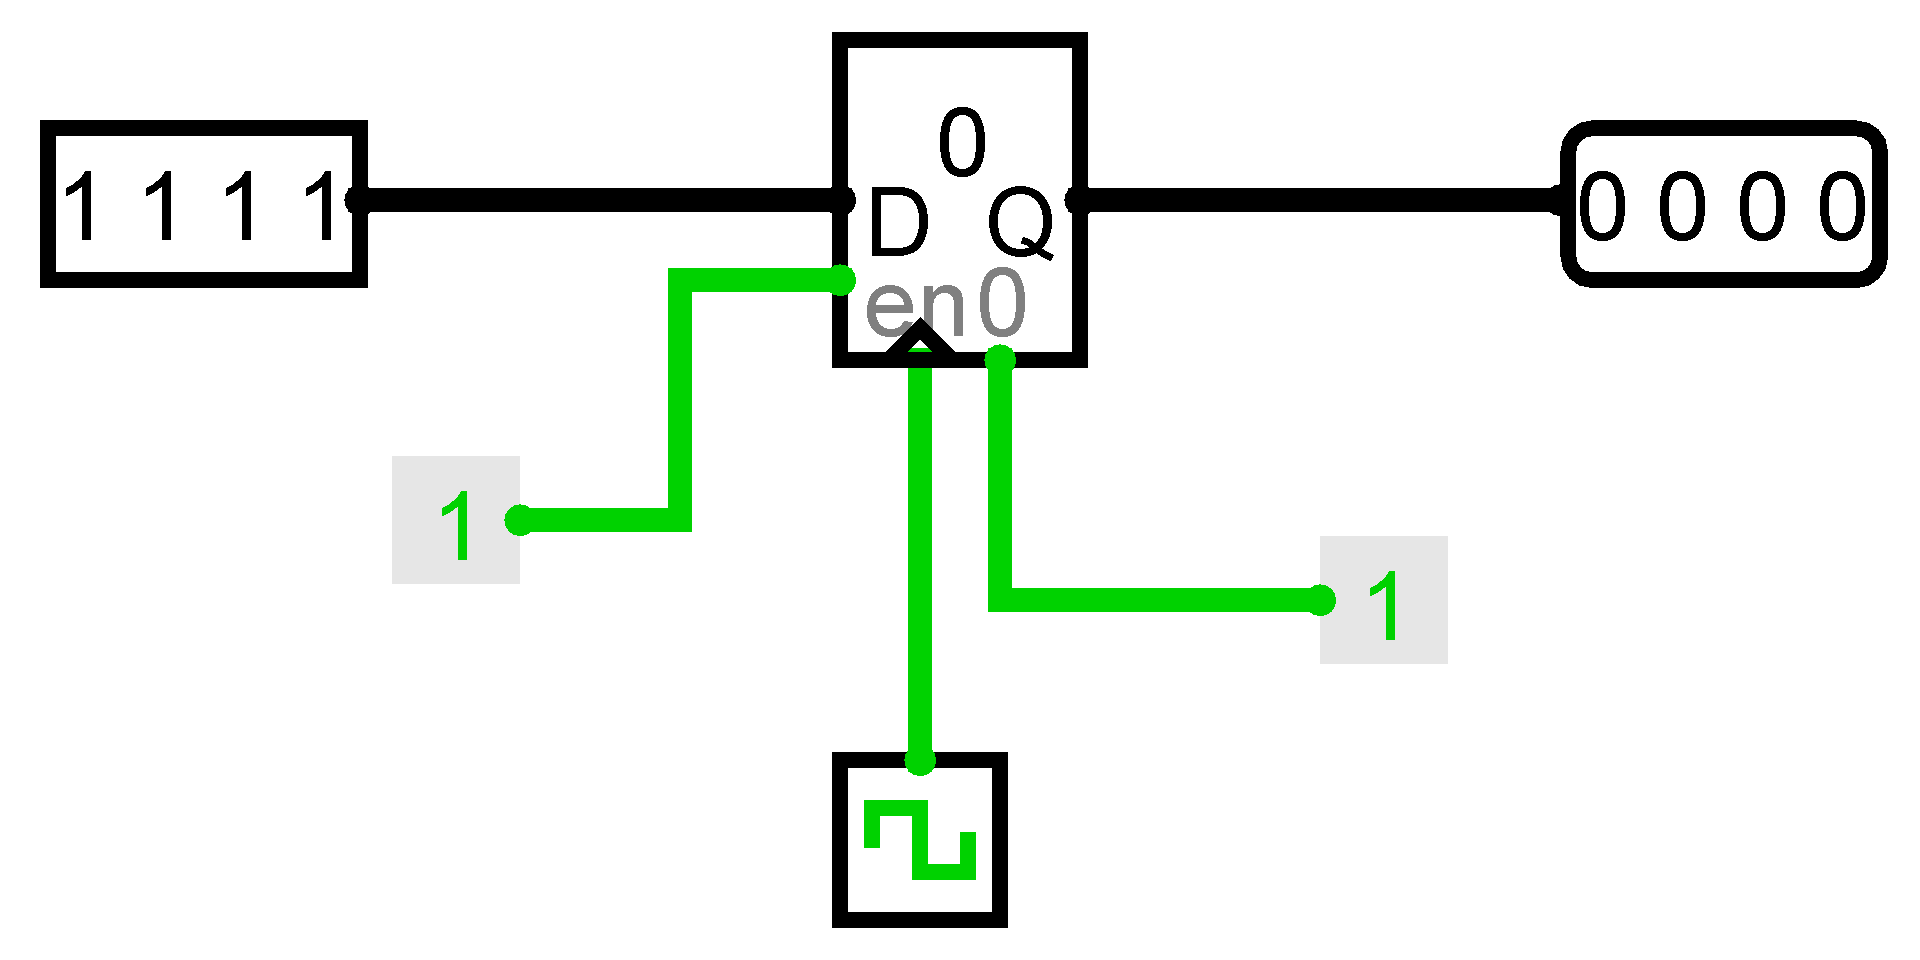
\includegraphics[width=0.6\textwidth]{img/cuartotry.png}
        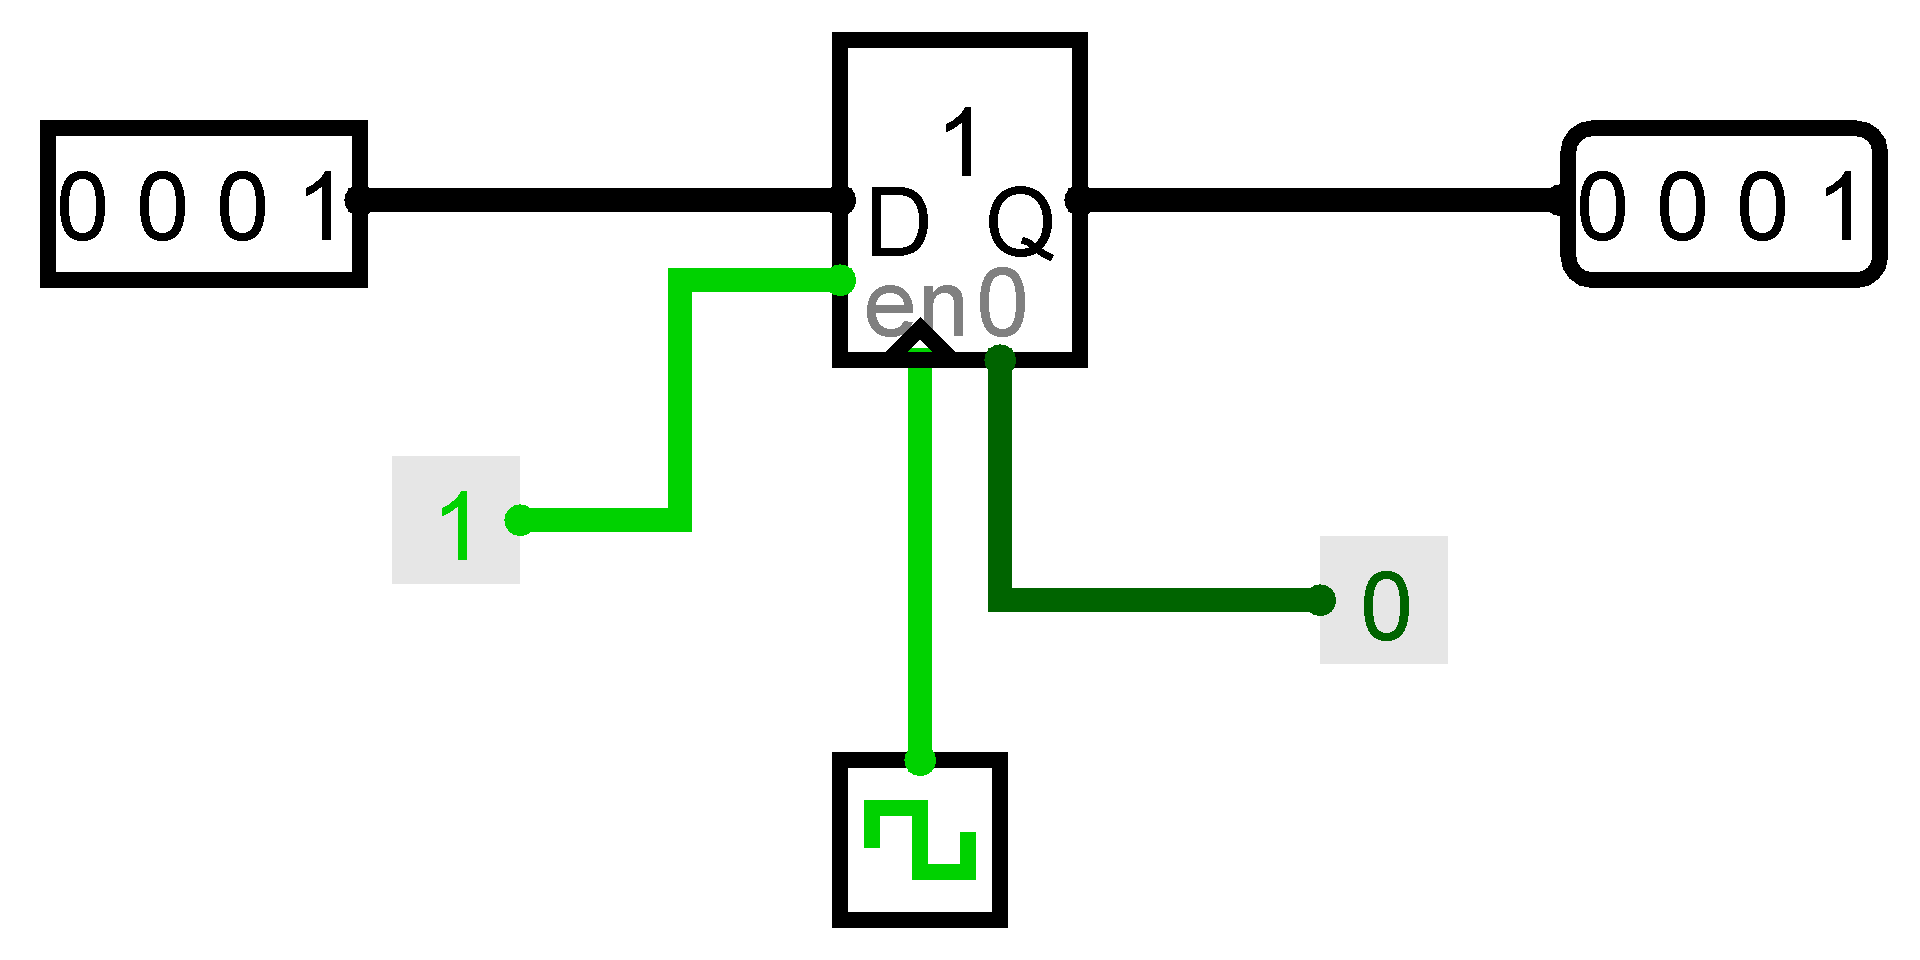
\includegraphics[width=0.6\textwidth]{img/quintotry.png}
    \end{figure}

    \item ¿Para qué nos sirve operar en los pines ENABLE y RESET? Pruebe funcionamiento. 
    
    Los pines ENABLE y RESET controlan el estado del registro. Cuando ENABLE tiene un valor de 1, el registro se habilita y puede almacenar los valores de entrada. Si RESET tiene un valor de 1, el registro se resetea y se pone en 0. En resumen, ENABLE permite que el registro funcione y almacene datos, mientras que RESET lo borra, poniendo todos los valores en 0.
    En el siguiente ejemplo se muestra lo que sucede con ENABLE en 1 y RESET en 0.

    \begin{figure}[H]
        \centering
        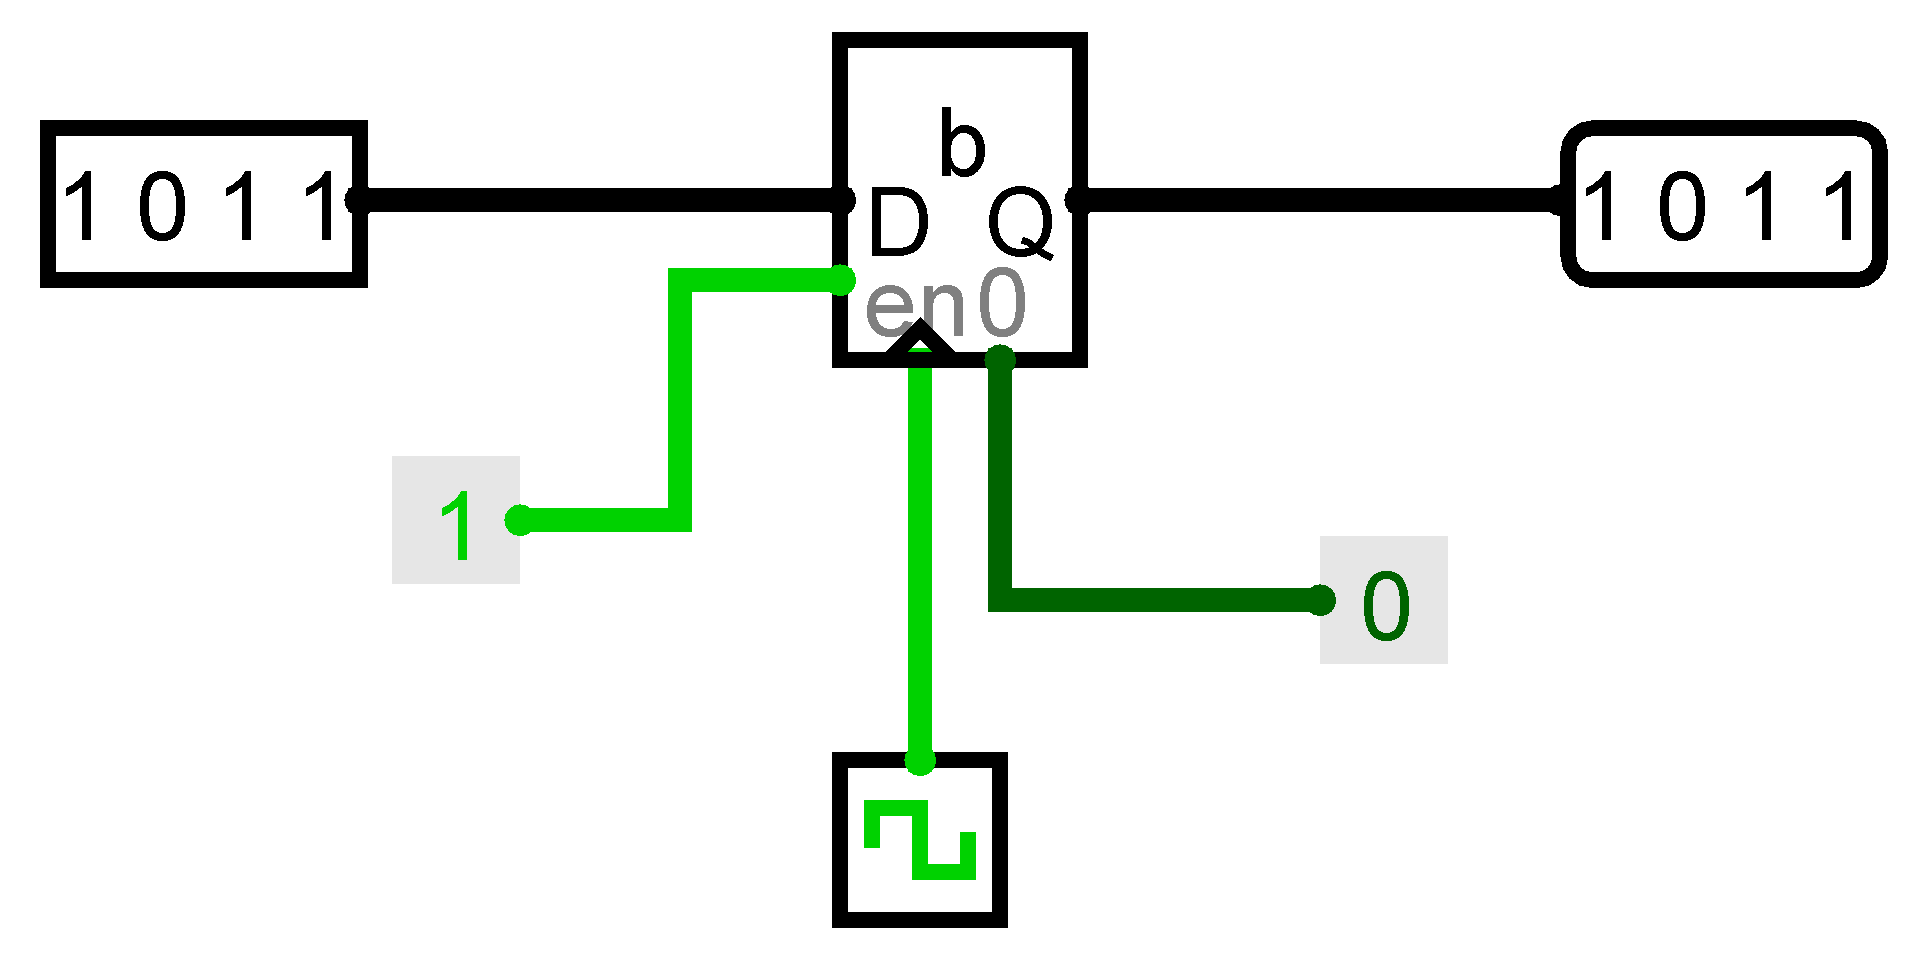
\includegraphics[width=0.6\textwidth]{img/enable.png}
    \end{figure}

    Sin embargo para el siguiente caso se tiene en valor 1 el pin RESET y se puede ver que el registro se resetea y se pone en 0 mientras este valor se mantenga en 1.

    \begin{figure}[H]
        \centering
        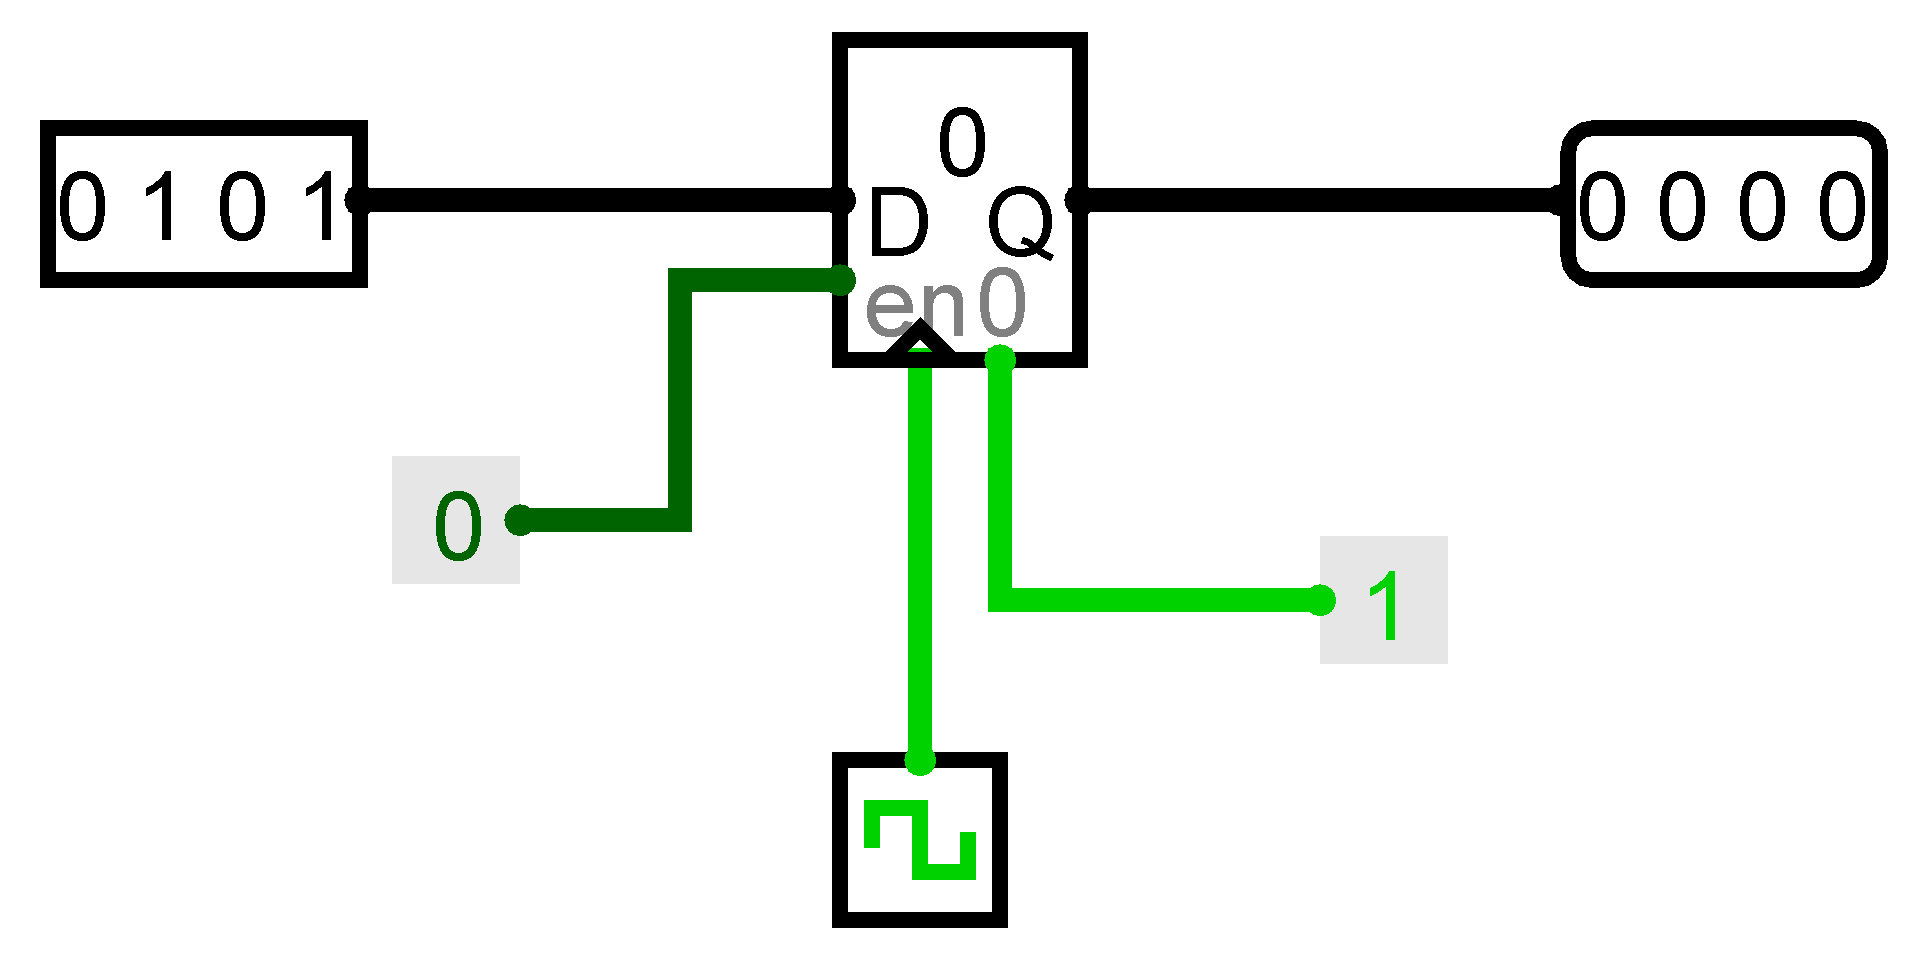
\includegraphics[width=0.6\textwidth]{img/reset.png}
    \end{figure}
    
    \item ¿Cómo puede el registro operar como Latch?

    El registro puede operar como Latch si se conecta el pin ENABLE a 1 y el pin RESET a 0. De esta forma, el registro se habilita y puede almacenar los valores de entrada, pero no se resetea. Por lo tanto, el registro se comporta como un Latch, ya que mantiene los valores almacenados en la entrada.
    
\end{enumerate}


\end{document}